\usetikzlibrary{arrows, positioning}

\begin{frame}
  \frametitle{Source Separation to Sequential Prediction}
  \begin{block}{Discrete Resonance Spectrogram}
    \textbf{TODO}: (Insert wide aspect ratio image of DRS)
  \end{block}
  \begin{block}{From Vertical to Horizontal Analysis}
    \begin{itemize}
      \item Source separation looks at dependencies between frequencies \textbf{within a slice}, i.e. vertical analysis.
      \item Temporal correlations can be exploited to observe dependencies \textbf{between slices}, i.e. horizontal analysis.
    \end{itemize}
  \end{block}
\end{frame}

\begin{frame}
  \frametitle{Boundary Entropy Segmentation}
  \begin{block}{Boundary Entropy}
    \begin{itemize}
      \item Intuition
      \item Unexpectedness
      \item Uncertainty
    \end{itemize}
  \end{block}
  \begin{block}{Hierarchical Chunking}
    \includegraphics[width=\textwidth]{images/phonetic-sequential-memory.png}
  \end{block}
\end{frame}

\begin{frame}
  \frametitle{Sequence vs Network Interpretation of BES}
  \begin{columns}
    \begin{column}{0.5\textwidth}
      \begin{block}{Sequence Interpretation}
        \centering
        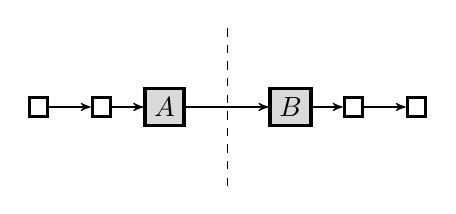
\begin{tikzpicture}[>= stealth', auto, scale=0.8]
          \tikzstyle{node}=[rectangle, very thick, draw=black]

          \node[node, fill=black!15] at (0,0) (A) {$A$};
          \node[node, fill=black!15] at (2,0) (B) {$B$};
          \node[node] (X1) at (-2,0) {};
          \node[node] (X2) at (-1,0) {};
          \node[node] (Y1) at (3,0) {};
          \node[node] (Y2) at (4,0) {};

          \path (X1) edge[->] (X2);
          \path (X2) edge[->] (A);
          \path (A) edge[->] (B);
          \path (B) edge[->] (Y1);
          \path (Y1) edge[->] (Y2);

          \draw[dashed] (1,1.25) -- (1,-1.25);

        \end{tikzpicture}
        \begin{itemize}
          \item
          \item
          \item
        \end{itemize}
      \end{block}
    \end{column}
    \begin{column}{0.5\textwidth}
      \begin{block}{Network Interpretation}
        \centering
        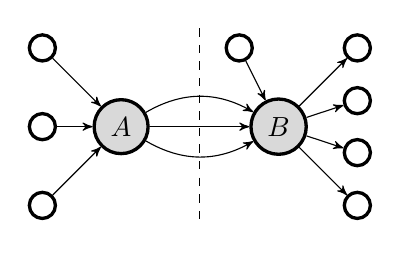
\begin{tikzpicture}[>= stealth', auto]
          \tikzstyle{node}=[circle, very thick, draw=black]

          \node[node, fill=black!15] at (0,0) (A) {$A$};
          \node[node, fill=black!15] at (2,0) (B) {$B$};
          \node[node] (X2) at (-1,0) {};
          \node[node] (X1) at (-1,1) {};
          \node[node] (X3) at (-1,-1) {};
          \node[node] (Y2) at (3,1) {};
          \node[node] (Y1) at (3,0.33) {};
          \node[node] (Y3) at (3,-0.33) {};
          \node[node] (Y4) at (3, -1) {};
          \node[node] (Z) at (1.5, 1) {};

          \path (X1) edge[->] (A);
          \path (X2) edge[->] (A);
          \path (X3) edge[->] (A);
          \path (A) edge[->] (B);
          \path (A) edge[->] [bend left] (B);
          \path (A) edge[->] [bend right] (B);
          \path (Z) edge[->] (B);
          \path (B) edge[->] (Y1);
          \path (B) edge[->] (Y2);
          \path (B) edge[->] (Y3);
          \path (B) edge[->] (Y4);

          \draw[dashed] (1,1.25) -- (1,-1.25);

        \end{tikzpicture}
        \begin{itemize}
          \item
          \item
          \item
        \end{itemize}
      \end{block}
    \end{column}
  \end{columns}
\end{frame}

\begin{frame}
  \frametitle{Hierarchical Structure and Dynamics}
  \begin{columns}
    \begin{column}{0.5\textwidth}
      \begin{block}{Hierarchical Prediction}
          \includegraphics[width=\textwidth]{images/idyot-seqmem-graph-model.png}
      \end{block}
    \end{column}
    \begin{column}{0.5\textwidth}
      \begin{block}{Hierarchical Structure}
          \includegraphics[width=\textwidth]{images/hierarchical-block-model.png}
      \end{block}
    \end{column}
  \end{columns}
\end{frame}

\begin{frame}
  \frametitle{Memory Consolidation and the MDL Principle}
  \begin{block}{What is it?}
    \begin{itemize}
      \item
      \item
      \item
    \end{itemize}
  \end{block}
  \begin{block}{What does it mean?}
    \begin{itemize}
      \item
      \item
      \item
    \end{itemize}
  \end{block}
\end{frame}

\begin{frame}
  \frametitle{Placement and Next Steps}
  \begin{block}{Placement}
    \begin{itemize}
      \item 
      \item 
      \item 
    \end{itemize}
  \end{block}
  \begin{block}{Next Steps}
    \begin{itemize}
      \item 
      \item
      \item
    \end{itemize}
  \end{block}
\end{frame}

\begin{frame}
  \frametitle{Applications and Future Work}
  \begin{block}{Applications}
    \begin{itemize}
      \item 
      \item 
      \item 
    \end{itemize}
  \end{block}
  \begin{block}{Future Work}
    \begin{itemize}
      \item 
      \item
      \item
    \end{itemize}
  \end{block}
\end{frame}
